\documentclass[12pt]{article}
\usepackage{graphicx} % Required for inserting images
\usepackage{float}
\usepackage{listings}
\usepackage[dvipsnames]{xcolor}
\usepackage{geometry}
\usepackage[UTF8]{ctex}
\usepackage{amsmath}
\usepackage{amssymb}
\usepackage{mathrsfs,mathtools}
\usepackage{multirow}
\usepackage[english]{babel} % English language/hyphenation
\usepackage{tikz}
\usetikzlibrary{shapes,arrows,positioning}% Draw tree

\lstset{language=Python,
  breaklines=true,
  keywordstyle=\color{blue}\bfseries,
  showstringspaces=false,
  basicstyle=\footnotesize,
  frame = single}


\title{Operations Reasearch, Spring 2024 (112-2)\\ Homework 2}
\author{B10705034 資管三\ 許文鑫}
\geometry{a4paper,scale=0.85}
\begin{document}
\maketitle
\begin{enumerate}
      \item (20 points; 5 points each) Consider the following LP
            \begin{align*}
                  \min \quad        & x_1 + 3x_2                        \\
                  \text{s.t.} \quad & x_1 + x_2 \geq 4                  \\
                                    & x_1 + 2x_2 \leq 9                 \\
                                    & x_2 \geq 3                        \\
                                    & x_i \geq 0 \quad \forall i = 1,2.
            \end{align*}
            \begin{enumerate}
                  \item Find the standard form of this LP.\\
                        \textbf{Ans.}
                        \begin{equation*}
                              \begin{alignedat}{10}
                                    \min \quad       &  & x_1 & \ +\  & 3x_2             \\
                                    \text{s.t.} \quad &  & x_1 & \ +\  & x_2  & \ -\  & x_3 &&&&& \ =\  & 4 \\
                                    && x_1 & \ +\  & 2x_2 & & &\ +\  & x_4 & & & \ =\  & 9\\
                                    && & & x_2 & & & & & \ -\  & x_5 & \ =\  & 3 \\
                                    & \mathrlap{x_i \geq 0\quad \forall i=1,\dots ,5.}
                              \end{alignedat}
                        \end{equation*}
                  \item List all the basic solutions and basic feasible solutions for the standard form of this LP.\\
                        \textbf{Ans.}\\
                        All the baif solutions and basic feasible solutions for the standard form of this LP are shown in Table \ref{tab:1}.
                        \begin{table}[H]
                              \centering
                              \begin{tabular}{|c|c|c|c|c|c|c|}
                                    \hline
                                    \multirow{2}{*}{Basis} & \multirow{2}{*}{feasible} & \multicolumn{5}{|c|}{Basic Solution}                                 \\
                                    \cline{3-7}            &                           & $x_1$                                & $x_2$ & $x_3$ & $x_4$ & $x_5$ \\
                                    \hline
                                    $(x_1,x_2,x_3)$        & Yes                       & 3                                    & 3     & 2     & 0     & 0     \\
                                    $(x_1,x_2,x_4)$        & Yes                       & 1                                    & 3     & 0     & 2     & 0     \\
                                    $(x_1,x_2,x_5)$        & No                        & -1                                   & 5     & 0     & 0     & 2     \\
                                    $(x_1,x_3,x_5)$        & No                        & 9                                    & 0     & 5     & 0     & -3    \\
                                    $(x_1,x_4,x_5)$        & No                        & 4                                    & 0     & 0     & 5     & -3    \\
                                    $(x_2,x_3,x_4)$        & No                        & 0                                    & 3     & -1    & 3     & 0     \\
                                    $(x_2,x_3,x_5)$        & Yes                       & 0                                    & 4.5   & 0.5   & 0     & 1.5   \\
                                    $(x_2,x_4,x_5)$        & Yes                       & 0                                    & 4     & 0     & 1     & 1     \\
                                    $(x_3,x_4,x_5)$        & No                        & 0                                    & 0     & -4    & 9     & -3    \\
                                    \hline
                              \end{tabular}
                              \caption{All the basic solutions and basic feasible solutions for the LP.}
                              \label{tab:1}
                        \end{table}

                  \item List all the extreme points of the feasible region of the original LP. DO NOT prove that they are extreme points; just list them. Then show that there is a one-to-one correspondence between basic feasible solutions and extreme points.\\
                        \textbf{Ans.}\\
                        basic feasible solutions:
                        \begin{equation*}
                              (3,3,2,0,0), (1,3,0,2,0),(0,9,5,0,6)
                        \end{equation*}
                        extreme points:
                        \begin{equation*}
                              (3,3,2,0,0), (1,3,0,2,0),(0,9,5,0,6)
                        \end{equation*}
                        There is a one-to-one correspondence between basic feasible solutions and extreme points.
                  \item Use the simplex method (with the two-phase implementation, if needed) and the smallest index rule to solve the LP. Write down the complete process, optimal solution to the original LP, and its associated objective value. Is there any iteration that has no improvement?\\
                        \textbf{Ans.}\\
                        Its Phase-I standard form LP is
                        \begin{equation*}
                              \begin{alignedat}{14}
                                    \min \quad       &  &  &  &  &&&&&&&&x_6&\ +\ &x_7            \\
                                    \text{s.t.} \quad &  & x_1 & \ +\  & x_2  & \ -\  & x_3 &&&&&\ +\ &x_6&&& \ =\  & 4 \\
                                    && x_1 & \ +\  & 2x_2 & & &\ +\  & x_4 & & &&&&& \ =\  & 9\\
                                    && & & x_2 & & & & & \ -\  & x_5 &&&\ +\ &x_7& \ =\  & 3 \\
                                    & \mathrlap{x_i \geq 0\quad \forall i=1,\dots ,7.}
                              \end{alignedat}
                        \end{equation*}
                        The initial tableau is shown below.
                        \begin{table}[H]
                              \centering
                              \begin{tabular}{ccccccc|c}
                                    0 & 0 & 0  & 0 & 0  & -1 & -1 & 0       \\
                                    \hline
                                    1 & 1 & -1 & 0 & 0  & 1  & 0  & $x_6=4$ \\
                                    1 & 2 & 0  & 1 & 0  & 0  & 0  & $x_4=9$ \\
                                    0 & 1 & 0  & 0 & -1 & 0  & 1  & $x_7=3$ \\
                              \end{tabular}
                        \end{table}
            \end{enumerate}
            Adjust the tableau to get the following tableau.
            \begin{table}[H]
                  \centering
                  \begin{tabular}{ccccccc|c}
                        1 & 2 & -1 & 0 & -1 & 0 & 0 & 7       \\
                        \hline
                        1 & 1 & -1 & 0 & 0  & 1 & 0 & $x_6=4$ \\
                        1 & 2 & 0  & 1 & 0  & 0 & 0 & $x_4=9$ \\
                        0 & 1 & 0  & 0 & -1 & 0 & 1 & $x_7=3$ \\
                  \end{tabular}
            \end{table}
            Solve the Phase-I LP:
            \begin{table}[H]
                  \centering
                  \begin{tabular}{cccccc|c}
                        0 & 1 & 0  & 0 & -1 & 0 & 3       \\
                        \hline
                        1 & 1 & -1 & 0 & 0  & 0 & $x_1=4$ \\
                        0 & 1 & 1  & 1 & 0  & 0 & $x_4=5$ \\
                        0 & 1 & 0  & 0 & -1 & 1 & $x_7=3$ \\
                  \end{tabular}
                  $\rightarrow$
                  \begin{tabular}{ccccc|c}
                        0 & 0 & 0  & 0 & 0  & 0       \\
                        \hline
                        1 & 0 & -1 & 0 & 1  & $x_1=1$ \\
                        0 & 0 & 1  & 1 & 1  & $x_4=2$ \\
                        0 & 1 & 0  & 0 & -1 & $x_2=3$ \\
                  \end{tabular}
            \end{table}
            A feasible basis for the original LP is $(x_1,x_2,x_4)$.
            Solve the phase-II LP:
            \begin{table}[H]
                  \centering
                  \begin{tabular}{ccccc|c}
                        -1 & -3 & 0  & 0 & 0  & 0       \\
                        \hline
                        1  & 0  & -1 & 0 & 1  & $x_1=1$ \\
                        0  & 0  & 1  & 1 & 1  & $x_4=2$ \\
                        0  & 1  & 0  & 0 & -1 & $x_2=3$ \\
                  \end{tabular}
                  $\xrightarrow{\text{Adjust}}$
                  \begin{tabular}{ccccc|c}
                        0 & 0 & -1 & 0 & -2 & 10      \\
                        \hline
                        1 & 0 & -1 & 0 & 1  & $x_1=1$ \\
                        0 & 0 & 1  & 1 & 1  & $x_4=2$ \\
                        0 & 1 & 0  & 0 & -1 & $x_2=3$ \\
                  \end{tabular}
            \end{table}
            The optimal bfs is $(1,3,0,2,0)$, where the objective value is 10.
      \item (10 points; 5 points each) Consider the integer program
            \begin{align*}
                  \max \quad       & 2x_1 + 2x_2 + 5x_3 + 11x_4 + 10x_5+3x_6 -6x_7       \\
                  \text{s.t.}\quad & x_1 + 4x_2 + 3x_3 + 5x_4 + 3x_5 -4x_6 + 2x_7 \leq 6 \\
                                   & x_i \in \{0,1\} \quad \forall i = 1,...,7,
            \end{align*}
            which is a variant of the knapsack problem.
            \begin{enumerate}
                  \item Use the greedy algorithm introduced in class to solve the linear relaxation of this integer program.\\
                        \textbf{Ans.}\\
                        The relaxation is:
                        \begin{align*}
                              \max \quad       & 2x_1 + 2x_2 + 5x_3 + 11x_4 + 10x_5+3x_6 -6x_7       \\
                              \text{s.t.}\quad & x_1 + 4x_2 + 3x_3 + 5x_4 + 3x_5 -4x_6 + 2x_7 \leq 6 \\
                                               & x_i \in [0,1] \quad \forall i = 1,...,7,
                        \end{align*}
                        Ane the ratio of the coefficients to the constraint is:
                        \begin{equation*}
                              \begin{aligned}
                                    \frac{2}{1} = 2, \frac{2}{4} = 0.5, \frac{5}{3} = 1.67, \frac{11}{5} = 2.2, \frac{10}{3} = 3.33, \frac{3}{-4} = -0.75, \frac{-6}{2} = -3
                              \end{aligned}
                        \end{equation*}
                        We pick from the largest ratio to the smallest ratio,and pick $x_6$ since its coefficeients is positive and the constraint is negative.
                        \begin{equation*}
                              x_1 = 1,x_2 = 0,x_3 = \frac{1}{3},x_4=1,x_5 = 1,x_6 = 1, x_7 = 0
                        \end{equation*}
                        and the objective value is $\frac{83}{3}$.
                  \item Use the branch-and-bound algorithm to solve the original integer program. Depict the full branch-and-bound tree. Do not write down the solution process of each node; write down just an optimal solution and its objective value of each node.\\
                        \textbf{Ans.}\\
                        \begin{figure}
                              \centering
                              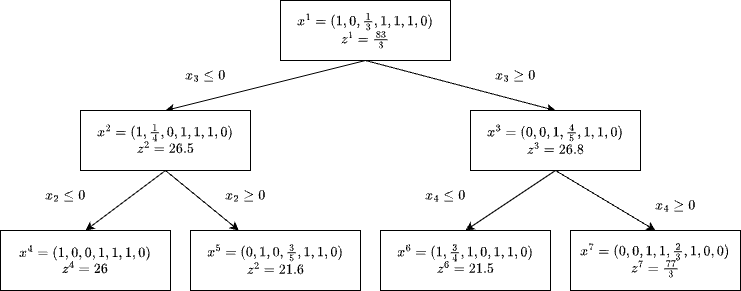
\includegraphics[scale=0.5]{2_b.png}
                        \end{figure}
            \end{enumerate}
            $x^3$ is optimal solution and $z^3 = 26$.
      \item (15 points) There are $m$ towns in a county. The county government is considering where to build at least $p$ landfills in $n$ potential locations. The distance between town $i$ and location $j$ is $d_{ij}$ . The population at town $i$ is $h_i$. The government wants to maximize the average distances between each person and her/his closest landfill.
            \begin{enumerate}
                  \item (5 points) Formulate an integer program to achieve this goal. Use your own words to explain the formulation in details.\\
                        \textbf{Hint.} This problem has appeared in one lecture problem.\\
                        \textbf{Note.} If you believe ChatGPT may help you explain the formulation, please feel free to use it. All you need to do is to make sure that the explanation is correct, precise, and concise.\\
                        \textbf{Ans.}\\
                        Let $J =\{1,\dots,n\}$ be the potential locations and $I = \{1,\dots, m\}$ be the set of towns.\\
                        Let $x_j = 1$ if a landfill is built at location $j$ and $x_j = 0$ otherwise.\\
                        Let $w_i$ be the distance between town $i$ and its closest landfill.
                        \begin{align}
                              \max \quad       & \sum_{i=1}^m h_iw_i                                           \\
                              \text{s.t.}\quad & \sum_{j=1}^n x_j \geq p                                       \\
                                               & w_i \leq d_{ij}x_j + M_i(1-x_j) \quad \forall i \in I, j\in J \\
                                               & x_j \in \{0,1\} \quad \forall j \in J,                        \\
                                               & w_i \geq 0 \quad \forall i \in I
                        \end{align}
                        Where $M_i$ is a large number. We can set $M_i = \max_{j\in J}\{d_{ij}\}\quad \forall i \in I$.\\
                        (1) is the objective function to maximize the average distances between each person and her/his closest landfill.\\
                        (2) is the constraint that the number of landfills built is at least $p$.\\
                        (3) is the constraint that
                        $w_i$ is the distance between town $i$ and its closest landfill. If $x_j = 1$, then $w_i \leq d_{ij}$, otherwise $w_i \leq M$.\\
                        (4) is the constraint that $x_j$ is binary.
                        (5) is the constraint that $w_i$ is non-negative.
                  \item (10 points) Consider the two instances contained in the file "OR112-2 hw02 data.xlsx" (if you do not use Microsoft Excel, you may use Google Spreadsheet to open the file). In each sheet, which contains an instance, parameter symbols are in blue cells, indices are in orange cells, and parameter values are in green cells. For example, in instance $2$, $m = 20, n = 10, p = 5, h_2 = 28,$ and $d_{12,5} = 164$.\\
                        Write Python to invoke Gurobi Optimizer to solve the two instances. Submit your Python
                        program by copying and pasting it into your answer. You should not hard code those parameter values; please put the parameter values in a file and read data from the file to retrieve
                        the values. There is no need to explain the program in your answer; just submit it. Moreover,
                        report the optimal solutions (and their objective values) you find for the two instances.\\
                        If you prefer, you may write your program in other languages; if you prefer, you may use
                        other optimization library (as long as you ensure that it generates a correct optimal solution).
                        Nevertheless, please understand that while we provide instruction on using Python to invoke
                        Gurobi Optimizer, there is nothing we may help with other combinations.\\
                        \textbf{Ans.}\\
                        \textbf{Instance 1}:
                        \begin{lstlisting}[language=Python]
from gurobipy import *
import numpy as np
import pandas as pd
sheet = "Problem 3 Instance 1"
file = "OR112-2_hw02_data.xlsx"
model = Model(sheet)

m = pd.read_excel(file,usecols="B:B",nrows=1,sheet_name=sheet)
m = int(m.columns.item())
n = pd.read_excel(file,usecols="B:B",skiprows=range(1),nrows=1,sheet_name=sheet)
n = int(n.columns.item())
p = pd.read_excel(file,usecols="B:B",skiprows=range(2),nrows=1,sheet_name=sheet)
p = int(p.columns.item())

d = pd.read_excel(file,usecols="E:"+chr(ord('E')+n-1),skiprows=range(4),nrows=m,sheet_name=sheet)
d = d.to_numpy()

h = pd.read_excel(file,usecols="B:B",skiprows=range(4),nrows=m,sheet_name=sheet)
h = h.to_numpy()
                        \end{lstlisting}
                        Optimal solution:
                        \begin{align*}
                               & x_1 = 1,x_2 = 1,x_3 = 1,x_4 = 0,x_5 = 0              \\
                               & w_1 = 76, w_2 = 108, w_3 = 30, w_4 = 107, w_5 = 66,  \\
                               & w_6 = 121, w_7 = 29, w_8 = 95, w_9 = 56, w_{10} = 30
                        \end{align*}
                        Objective value:  $39027$\\
                        \textbf{Instance 2}:
                        \begin{lstlisting}[language=Python]
from gurobipy import *
import numpy as np
import pandas as pd
sheet = "Problem 3 Instance 2"
file = "OR112-2_hw02_data.xlsx"
model = Model(sheet)

m = pd.read_excel(file,usecols="B:B",nrows=1,sheet_name=sheet)
m = int(m.columns.item())
n = pd.read_excel(file,usecols="B:B",skiprows=range(1),nrows=1,sheet_name=sheet)
n = int(n.columns.item())
p = pd.read_excel(file,usecols="B:B",skiprows=range(2),nrows=1,sheet_name=sheet)
p = int(p.columns.item())

d = pd.read_excel(file,usecols="E:"+chr(ord('E')+n-1),skiprows=range(4),nrows=m,sheet_name=sheet)
d = d.to_numpy()

h = pd.read_excel(file,usecols="B:B",skiprows=range(4),nrows=m,sheet_name=sheet)
h = h.to_numpy()
x = model.addVars(n,vtype=GRB.BINARY, name="x")
w = model.addVars(m,vtype=GRB.INTEGER, name="w")

model.setObjective(quicksum(h[i][0]*w[i] for i in range(m)), GRB.MAXIMIZE)

model.addConstr(quicksum(x[i] for i in range(n)) >= p)
for i in range(m):
    for j in range(n):
        model.addConstr(w[i] <= d[i][j]*x[j]+np.max(d[i])*(1-x[j]))

model.optimize()
for v in model.getVars():
    print('%s %g' % (v.varName, v.x))
                        \end{lstlisting}
                        Optimal solution:
                        \begin{align*}
                               & x_1 = 1, x_2 = 0, x_3 = 1, x_4 = 0, x_5 = 1,                      \\
                               & x_6 = 0, x_7 = 1, x_8 = 1, x_9 = 0, x_{10} = 0.                   \\
                               & w_1 = 55, w_2 = 71, w_3 = 50, w_4 = 63, w_5 = 47,                 \\
                               & w_6 = 135, w_7 = 23, w_8 = 12, w_9 = 104, w_{10} = 19             \\
                               & w_{11} = 88, w_{12} = 27, w_{13} = 50, w_{14} = 37, w_{15} = 61,  \\
                               & w_{16} = 30, w_{17} = 28, w_{18} = 38, w_{19} = 98, w_{20} = 109.
                        \end{align*}
                        Objective value:  $68665$
            \end{enumerate}
      \item (35 points) Continue from Problem 3.
            \begin{enumerate}
                  \item (10 points) Consider the following greedy algorithm designed for the landfill location problem. The algorithm runs in $n - p$ iterations. Initially, the algorithm starts with a feasible solution that builds a landfill in each candidate locations. In each iteration, it examines all landfills to see if one and exactly one landfill can be removed, removing which one results in the maximum objective value in that iteration (and if there is a tie, it chooses the landfill with the smallest index). It keeps removing landfills until only $p$ landfills remain.\\
                        Implement this greedy algorithm in Python or any language you like. Submit your program by copying and pasting it into your answer. You should not hard code those parameter values; please put the parameter values in a file and read data from the file to retrieve the values. There is no need to explain the program in your answer; just submit it. Moreover, report the solutions (and their objective values) you find for the two instances.\\
                        \textbf{Ans.}\\
                        \textbf{Instance 1:}
                        \begin{lstlisting}[language=Python]
import numpy as np
import pandas as pd

sheet = "Problem 3 Instance 1"
file = "OR112-2_hw02_data.xlsx"

m = pd.read_excel(file,usecols="B:B",nrows=1,sheet_name=sheet)
m = int(m.columns.item())
n = pd.read_excel(file,usecols="B:B",skiprows=range(1),nrows=1,sheet_name=sheet)
n = int(n.columns.item())
p = pd.read_excel(file,usecols="B:B",skiprows=range(2),nrows=1,sheet_name=sheet)
p = int(p.columns.item())

d = pd.read_excel(file,usecols="E:"+chr(ord('E')+n-1),skiprows=range(4),nrows=m,sheet_name=sheet)
d = d.to_numpy()

h = pd.read_excel(file,usecols="B:B",skiprows=range(4),nrows=m,sheet_name=sheet)
h = h.to_numpy()

def objfunc(h,d,x):
    total = 0
    for i in range(h.shape[0]):
        total += h[i] * min(d[i,x.astype(bool)])
    return total.item()

    x = np.ones(n)
    for i in range(n-p):
        total = np.zeros(n)
        for j in range(n-i):
            tmp_x = x.copy()
            if tmp_x[j] == 1:
                tmp_x[j] = 0
                total[j] = objfunc(h,d,tmp_x)
        x[np.argmax(total)] = 0
    print(x)
    print(objfunc(h,d,x))    
                        \end{lstlisting}
                        Solution:
                        \begin{align*}
                               & x_1 = 1, x_2 = 1, x_3 = 1, x_4 = 0, x_5 = 0.         \\
                               & w_1 = 76, w_2 = 108, w_3 = 30, w_4 = 107, w_5 = 66,  \\
                               & w_6 = 121, w_7 = 29, w_8 = 95, w_9 = 56, w_{10} = 30
                        \end{align*}
                        Objective value:  $39027$\\
                        \textbf{Instance 2:}
                        \begin{lstlisting}[language=Python]
import numpy as np
import pandas as pd

sheet = "Problem 3 Instance 2"
file = "OR112-2_hw02_data.xlsx"

m = pd.read_excel(file,usecols="B:B",nrows=1,sheet_name=sheet)
m = int(m.columns.item())
n = pd.read_excel(file,usecols="B:B",skiprows=range(1),nrows=1,sheet_name=sheet)
n = int(n.columns.item())
p = pd.read_excel(file,usecols="B:B",skiprows=range(2),nrows=1,sheet_name=sheet)
p = int(p.columns.item())

d = pd.read_excel(file,usecols="E:"+chr(ord('E')+n-1),skiprows=range(4),nrows=m,sheet_name=sheet)
d = d.to_numpy()

h = pd.read_excel(file,usecols="B:B",skiprows=range(4),nrows=m,sheet_name=sheet)
h = h.to_numpy()

def objfunc(h,d,x):
      total = 0
      for i in range(h.shape[0]):
            total += h[i] * min(d[i,x.astype(bool)])
      return total.item()

      x = np.ones(n)
      for i in range(n-p):
            total = np.zeros(n)
            for j in range(n-i):
            tmp_x = x.copy()
            if tmp_x[j] == 1:
                  tmp_x[j] = 0
                  total[j] = objfunc(h,d,tmp_x)
            x[np.argmax(total)] = 0
      print(x)
      print(objfunc(h,d,x))    
                  \end{lstlisting}
                        Solution:
                        \begin{align*}
                               & x_1 = 0, x_2 = 1, x_3 = 0, x_4 = 1, x_5 = 0,                      \\
                               & x_6 = 1, x_7 = 0, x_8 = 0, x_9 = 1, x_{10} = 1.                   \\
                               & w_1 = 48, w_2 = 37, w_3 = 67, w_4 = 45, w_5 = 87,                 \\
                               & w_6 = 55, w_7 = 76, w_8 = 108, w_9 = 26, w_{10} = 107,            \\
                               & w_{11} = 37, w_{12} = 121, w_{13} = 29, w_{14} = 88, w_{15} = 56, \\
                               & w_{16} = 85, w_{17} = 100, w_{18} = 71, w_{19} = 7, w_{20} = 23.
                        \end{align*}
                        Objective value:  $65364$
                  \item (10 points) Consider another heuristic algorithm designed for the landfill location problem
                        based on linear relaxation. The idea is simple. Given an instance, first we solve its linear
                        relaxation to obtain a probably fractional LP-optimal solution $x^{LP}$ . We then pick the largest
                        $p$ values and set the corresponding $x^{LP}$ to 1 (if there is a tie, pick those with smaller indices);
                        the remaining $n - p$ variables are set to 0.\\
                        Implement this heuristic algorithm in Python or any language you like. When solving the linear relaxation, use Gurobi Optimizer or any optimization library you like. Submit your program by copying and pasting it into your answer. You should not hard code those param- eter values; please put the parameter values in a file and read data from the file to retrieve the values. There is no need to explain the program in your answer; just submit it. Moreover, report the solutions (and their objective values) you find for the two instances.\\
                        \textbf{Ans.}\\
                        \textbf{Instance 1:}
                        \begin{lstlisting}[language=Python]
from gurobipy import *
import numpy as np
import pandas as pd

def objfunc(h,d,x):
    total = 0
    for i in range(h.shape[0]):
        total += h[i] * min(d[i,x.astype(bool)])
    return total.item()


sheet = "Problem 3 Instance 1"
file = "OR112-2_hw02_data.xlsx"
model = Model(sheet)

m = pd.read_excel(file,usecols="B:B",nrows=1,sheet_name=sheet)
m = int(m.columns.item())
n = pd.read_excel(file,usecols="B:B",skiprows=range(1),nrows=1,sheet_name=sheet)
n = int(n.columns.item())
p = pd.read_excel(file,usecols="B:B",skiprows=range(2),nrows=1,sheet_name=sheet)
p = int(p.columns.item())

d = pd.read_excel(file,usecols="E:"+chr(ord('E')+n-1),skiprows=range(4),nrows=m,sheet_name=sheet)
d = d.to_numpy()

h = pd.read_excel(file,usecols="B:B",skiprows=range(4),nrows=m,sheet_name=sheet)
h = h.to_numpy()

x = model.addVars(n,lb=0.0,ub=1.0,vtype=GRB.CONTINUOUS, name="x")
w = model.addVars(m,vtype=GRB.CONTINUOUS, name="w")

model.setObjective(quicksum(h[i][0]*w[i] for i in range(m)), GRB.MAXIMIZE)

model.addConstr(quicksum(x[i] for i in range(n)) >= p)
for i in range(m):
      for j in range(n):
            model.addConstr(w[i] <= d[i][j]*x[j]+np.max(d[i])*(1-x[j]))

model.optimize()
x = []
for v in model.getVars():
      print('%s %g' % (v.varName, v.x))
      x.append(v.x)

x = x[:n]
tmp_x = np.zeros(n)
print(x)
for i in range(p):
    tmp_x[np.argmax(x)] = 1
    x[np.argmax(x)] = 0
print(tmp_x)
print(objfunc(h,d,tmp_x))
                        \end{lstlisting}
                        We first have $x^{LP}$:
                        \begin{align*}
                               & x_{0} = 0.5949548088466156,  \\
                               & x_{1} = 1.0,                 \\
                               & x_{2} = 0.7487071751777633,  \\
                               & x_{3} = 0.38062725090036004, \\
                               & x_{4} = 0.2757107650752609.
                        \end{align*}
                        Then apply the heuristic algorith, get
                        $\bar{x}$:
                        \begin{align*}
                               & x_{0} = 1, \\
                               & x_{1} = 1, \\
                               & x_{2} = 1, \\
                               & x_{3} = 0, \\
                               & x_{4} = 0.
                        \end{align*}
                        So the solution is:
                        \begin{align*}
                               & x_1 = 1, x_2 = 1, x_3 = 1, x_4 = 0, x_5 = 0.         \\
                               & w_1 = 76, w_2 = 108, w_3 = 30, w_4 = 107, w_5 = 66,  \\
                               & w_6 = 121, w_7 = 29, w_8 = 95, w_9 = 56, w_{10} = 30
                        \end{align*}
                        Objective value:  $39027$\\
                        \textbf{Instance 2:}
                        \begin{lstlisting}[language=Python]
from gurobipy import *
import numpy as np
import pandas as pd

def objfunc(h,d,x):
      total = 0
      for i in range(h.shape[0]):
            total += h[i] * min(d[i,x.astype(bool)])
      return total.item()


sheet = "Problem 3 Instance 2"
file = "OR112-2_hw02_data.xlsx"
model = Model(sheet)

m = pd.read_excel(file,usecols="B:B",nrows=1,sheet_name=sheet)
m = int(m.columns.item())
n = pd.read_excel(file,usecols="B:B",skiprows=range(1),nrows=1,sheet_name=sheet)
n = int(n.columns.item())
p = pd.read_excel(file,usecols="B:B",skiprows=range(2),nrows=1,sheet_name=sheet)
p = int(p.columns.item())

d = pd.read_excel(file,usecols="E:"+chr(ord('E')+n-1),skiprows=range(4),nrows=m,sheet_name=sheet)
d = d.to_numpy()

h = pd.read_excel(file,usecols="B:B",skiprows=range(4),nrows=m,sheet_name=sheet)
h = h.to_numpy()

x = model.addVars(n,lb=0.0,ub=1.0,vtype=GRB.CONTINUOUS, name="x")
w = model.addVars(m,vtype=GRB.CONTINUOUS, name="w")

model.setObjective(quicksum(h[i][0]*w[i] for i in range(m)), GRB.MAXIMIZE)

model.addConstr(quicksum(x[i] for i in range(n)) >= p)
for i in range(m):
      for j in range(n):
            model.addConstr(w[i] <= d[i][j]*x[j]+np.max(d[i])*(1-x[j]))

model.optimize()
x = []
for v in model.getVars():
      print('%s %g' % (v.varName, v.x))
      x.append(v.x)

x = x[:n]
tmp_x = np.zeros(n)
print(x)
for i in range(p):
      tmp_x[np.argmax(x)] = 1
      x[np.argmax(x)] = 0
print(tmp_x)
print(objfunc(h,d,tmp_x))
                        \end{lstlisting}
                        We first have $x^{LP}$:
                        \begin{align*}
                               & x_{1} = 0.47636549575898146, \\
                               & x_{2} = 0.444908809010339,   \\
                               & x_{3} = 0.433059541599074,   \\
                               & x_{4} = 0.4390081616759844,  \\
                               & x_{5} = 0.6125695279199782,  \\
                               & x_{6} = 0.5543705001160574,  \\
                               & x_{7} = 0.47559217514898305, \\
                               & x_{8} = 0.36340660833488725, \\
                               & x_{9} = 0.4909176989787073,  \\
                               & x_{10} = 0.7098014814570079.
                        \end{align*}
                        Then apply the heuristic algorith, get
                        $\bar{x}$:
                        \begin{align*}
                               & x_1 = 1,    \\
                               & x_2 = 0,    \\
                               & x_3 = 0,    \\
                               & x_4 = 0,    \\
                               & x_5 = 1,    \\
                               & x_6 = 1,    \\
                               & x_7 = 0,    \\
                               & x_8 = 0,    \\
                               & x_9 = 1,    \\
                               & x_{10} = 1.
                        \end{align*}
                        So the solution is:
                        \begin{align*}
                               & w_{1} = 79, w_{2} = 71, w_{3} = 50, w_{4} = 63, w_{5} = 87,      \\
                               & w_{6} = 55, w_{7} = 71, w_{8} = 41, w_{9} = 53, w_{10} = 62,     \\
                               & w_{11} = 37, w_{12} = 27, w_{13} = 91, w_{14} = 81, w_{15} = 77, \\
                               & w_{16} = 30, w_{17} = 76, w_{18} = 38, w_{19} = 38, w_{20} = 23.
                        \end{align*}
                        Objective value:  $63044$
                  \item (5 points) Let $z_k^G$ be the objective value of the solution found by the greedy algorithm in Part (a) for instance $k \in \{1,2\}$. Similarly, let $z_k^R$ be that by the heuristic algorithm in Part (b) for instance $k \in \{1, 2\}$. For each of the two instances, report $z_k^{IP}$ , $z_k^{LP}$ , $z_k^G$, $z_k^R$, and the four percentage optimality gaps (each algorithm has two optimality gaps, one uses $z_k^{IP}$ and one uses $z_k^{LP}$ ). In average, which algorithm performs better in these two instances?\\
                        \textbf{Ans.}\\
                        \textbf{Instance 1:}
                        \begin{equation*}
                              z^{IP}_k = 39072, z^{LP} _k= 53434.86724, z^{G}_k = 39027, z^{R}_k = 39027
                        \end{equation*}
                        \begin{table}[H]
                              \centering
                              \begin{tabular}{c|c|c|c}
                                    error     & $z^{IP}_k$ & $z^{LP}_k$ & average \\
                                    \hline
                                    $z^{G}_k$ & 0          & 0.2696     & 0.1348  \\
                                    \hline
                                    $z^{R}_k$ & 0          & 0.2696     & 0.1348  \\
                              \end{tabular}
                        \end{table}
                        \textbf{Instance 2:}
                        \begin{equation*}
                              z^{IP}_k = 68665, z^{LP}_k = 117810.4228, z^{G}_k = 65364, z^{R}_k = 63044
                        \end{equation*}
                        \begin{table}[H]
                              \centering
                              \begin{tabular}{c|c|c|c}
                                    error     & $z^{IP}_k$ & $z^{LP}_k$ & average \\
                                    \hline
                                    $z^{G}_k$ & 0.0481     & 0.4452     & 0.24665 \\
                                    \hline
                                    $z^{R}_k$ & 0.0819     & 0.4649     & 0.2734  \\
                              \end{tabular}
                        \end{table}
                        In average, the greedy algorithm performs better.
                  \item (10 points) Comment on the time complexity (with the big-O notation) and performance of the two heuristic algorithms. If you need to solve the landfill location problem with $m = 500, n = 100, \text{and } p = 20,$ which algorithm do you prefer? Why?\\
                        \textbf{Hint.} The complexity of using the simplex method to solve a linear program with $m$ constraints in roughly $O(m^3).$ Though the way Gurobi Optimizer solves a linear program is more complicated than just running the classic simplex method, the complexity is pretty much at the same order. To answer this problem, please use the $O(m^3)$ fact directly.\\
                        \textbf{Ans.}\\
                        I will choose greedy algorithm.\\
                        The time complexity of the greedy algorithm is $O((n-p)n^2m)$, ant the time complexity of linear relaxation is $O(n^3m^3)$ since there's roughly $nm$ constraints.\\
                        So the greedy algorithm is not only faster but also performs quite well.
            \end{enumerate}
      \item (20 points; 10 points each) Consider the following nonlinear program
            \begin{equation*}
                  \min 3x_1^2 + 2x_2^2 + 4x_1x_2 +6e^{x_1}+x_2
            \end{equation*}
            Later when needed, use numerical solutions rather than analytical solutions. For example, when solving $-x = e^x$, using any calculator or software to find $x = -0.567$ as a numerical solution is good enough. There is no need to analytically solve $-x = e^x$.
            \begin{enumerate}
                  \item Start from $(x_1,x_2) = (0,0)$ to run one iteration of the gradient descent method to solve this instance. In this iteration, move to the global minimum along the direction you choose. Write down the detailed process of the iteration.\\
                        \textbf{Ans.}\\
                        We have:
                        \begin{equation*}
                              \nabla f(x) = \begin{bmatrix}
                                    6x_1+4x_2 + 6e^{x_1} \\
                                    4x_2+ 4x_1+1
                              \end{bmatrix}
                        \end{equation*}
                        \begin{itemize}
                              \item Step 0: $x^0 = (0,0), f(x^0) = 6$
                              \item Step 1:
                                    \begin{align*}
                                           & \nabla f(x^0) = \begin{bmatrix}
                                                                   6 \\
                                                                   1
                                                             \end{bmatrix}
                                           &                                                                        \\
                                           & a_0 =           \text{argmin}_{a>0}f(x^0-a\nabla f(x^0)),\text{where } \\
                                           & f(x^0-a\nabla f(x^0)) = f(-6a,-a)                                      \\
                                           & = 134a^2+6e^{-6a}-a, a_0=0.0846                                        \\
                                           & \text{Therefore, } x^1 = \begin{bmatrix}
                                                                            -0.5076 \\
                                                                            -0.0846
                                                                      \end{bmatrix}, \text{and }f(x^1) = 4.4861
                                    \end{align*},

                        \end{itemize}
                        Use python to solve $a$:
                        \begin{lstlisting}
from scipy.optimize import fsolve
import numpy as np

def func(a):
    return 268*a - 36*np.exp(-6*a) - 1

initial_guess = 0.1
solution = fsolve(func, initial_guess)

print(f"The solution is a = {solution[0]}")
                        \end{lstlisting}
                  \item Start from $(x_1, x_2) = (0, 0)$ to run one iteration of the Newton's method to solve this instance. Write down the detailed process of the iteration.\\
                        \textbf{Ans.}
                        \begin{equation*}
                              \text{Hessian:}
                              \begin{bmatrix}
                                    6+6e^{x_1} & 4 \\
                                    4          & 4
                              \end{bmatrix}
                        \end{equation*}
                        \begin{align*}
                              x^1 = x^0 - [\nabla^{2}f(x^0)\nabla]^{-1} f(x^0) = \begin{bmatrix}
                                                                                       0 \\
                                                                                       0
                                                                                 \end{bmatrix} - \begin{bmatrix}
                                                                                                       0.625 \\
                                                                                                       -0.375
                                                                                                 \end{bmatrix} = \begin{bmatrix}
                                                                                                                       -0.625 \\
                                                                                                                       0.375
                                                                                                                 \end{bmatrix}
                        \end{align*}
                        Use python to solve:
                        \begin{lstlisting}
import numpy as np

def objfunc(x_1,x_2):
    return 3*pow(x_1,2) + 2*pow(x_2,2) +4*x_1*x_2 +6*np.exp(x_1) + x_2

x_1 = 0
x_2 = 0

hessian = np.array([[6 + 6*np.exp(x_1), 4], [4, 4]])
gradient = np.array([6*x_1 + 4*x_2 + 6*np.exp(x_1), 4*x_2 + 4*x_1+1])

inv_matrix = np.linalg.inv(hessian)
x = np.dot(inv_matrix, gradient)
print(x)

print(objfunc(x_1-x[0],x_2-x[1]))
                  \end{lstlisting}
                        The objective value is 4.1022.
            \end{enumerate}
\end{enumerate}
\end{document}